

\preClass{Integral Calculus Review}

\begin{problem}
\item Find the solutions to the following integrals. In each case
  solve for $y$ in terms of $t$. (Do not forget the ``$+C$'' for each
  integral!)
  \begin{subproblem}
    \item $y = \int \cos(3t) ~ dt$
      \vfill
    \item $y = \int t^2 + e^{5t} ~ dt$
      \vfill
    \item $t = \int \frac{1}{y} ~ dy$
      \vfill
    \item $t = \int y^2 ~ dy$
      \vfill
  \end{subproblem}  
\end{problem}


\actTitle{Basic Integrals and Slope Fields}
\begin{problem}
\item Find the solutions to the following integrals. In each case
  solve for $y$ in terms of $t$. (Do not forget the ``$+C$'' for each
  integral!)
  \begin{subproblem}
    \item $y = \int t\cos(3t) ~ dt$
      \vfill
    \item $y = \int t e^{5t} ~ dt$
      \vfill
    \item $y = \int t^2 \ln(t) ~ dt$
      \vfill
    \item $t = \int \frac{\ln(y)}{y} ~ dy$
      \vfill
  \end{subproblem}

\clearpage

\item For each slope field make sketches for different solutions for
  each of the following initial conditions:
  \begin{eqnarray*}
    y(0) & = & 3, \\
    y(0) & = & 1, \\
    y(0) & = & 0, \\
    y(0) & = & -1, \\
    y(0) & = & -3.
  \end{eqnarray*}
  For each slope field state the general behavior and state the long
  term solutions if they exist.

  \begin{subproblem}
    \item 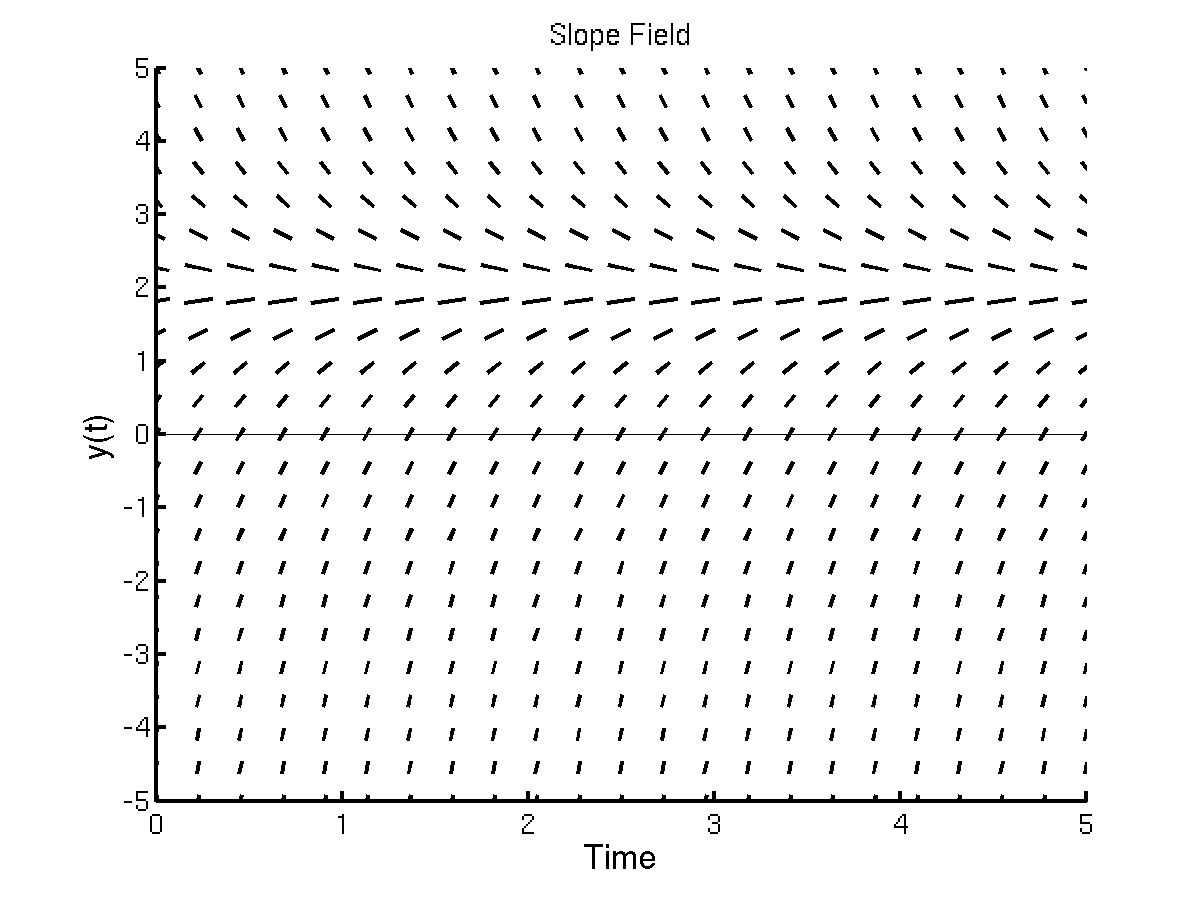
\includegraphics[height=3.0in]{sfSteadyWk1}
    \item 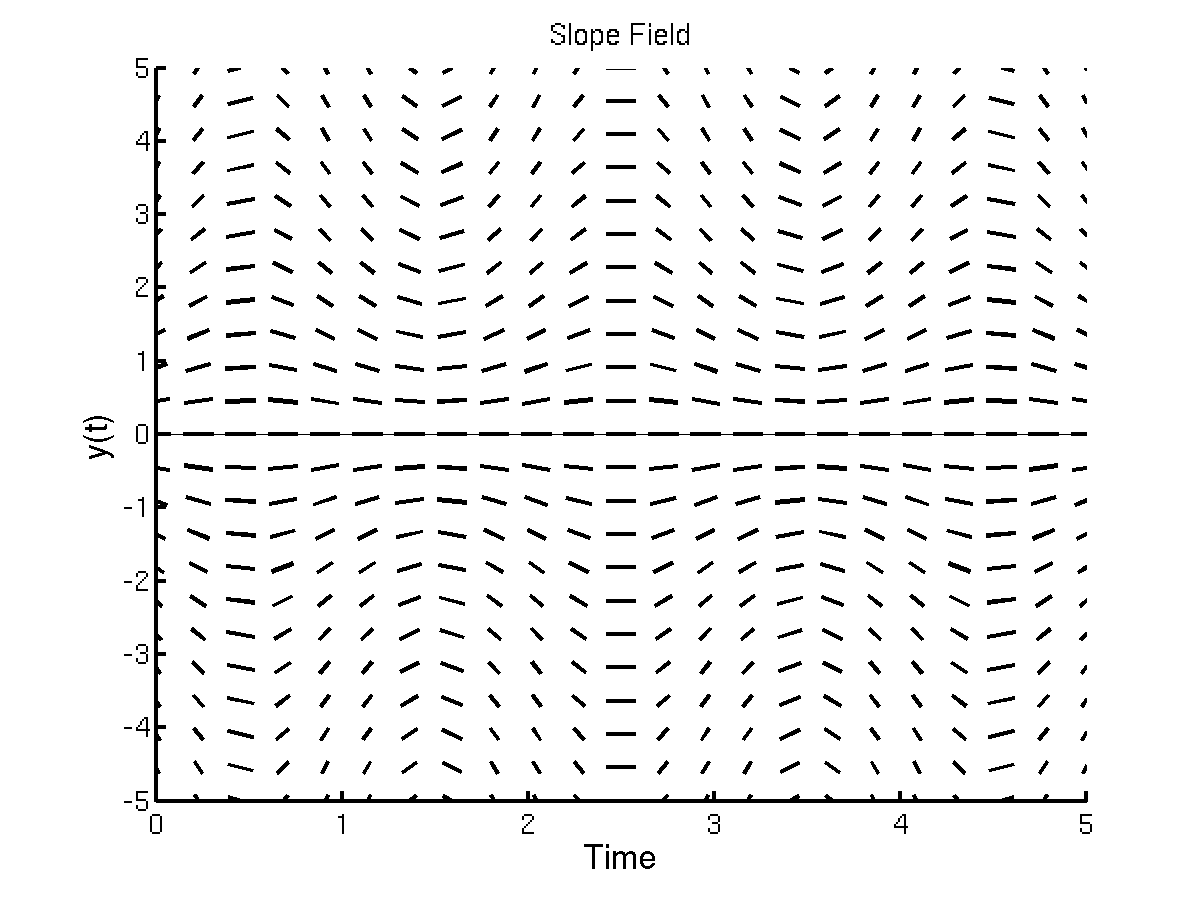
\includegraphics[height=3.0in]{sfOscillateWk1}

      \clearpage

    \item 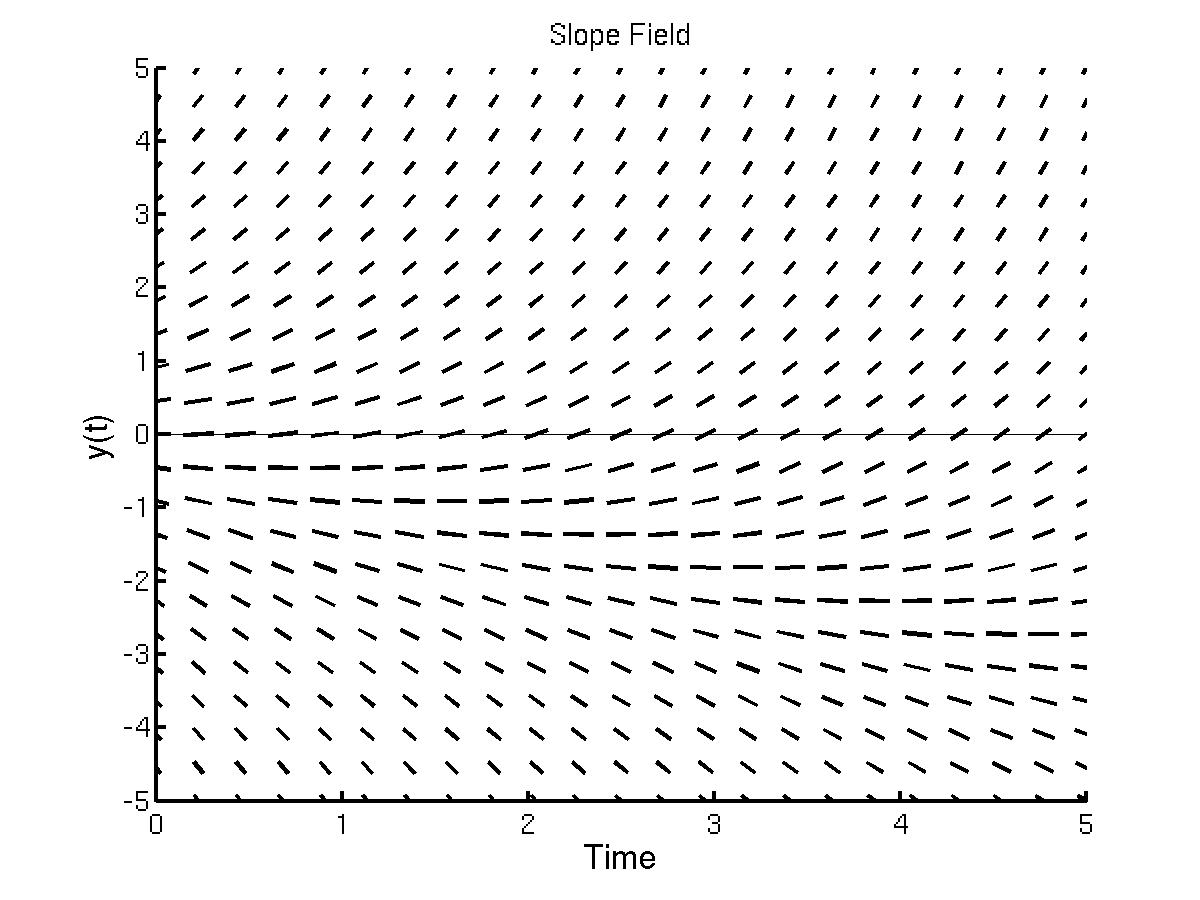
\includegraphics[height=4.0in]{sfLinearWk1}
    \item 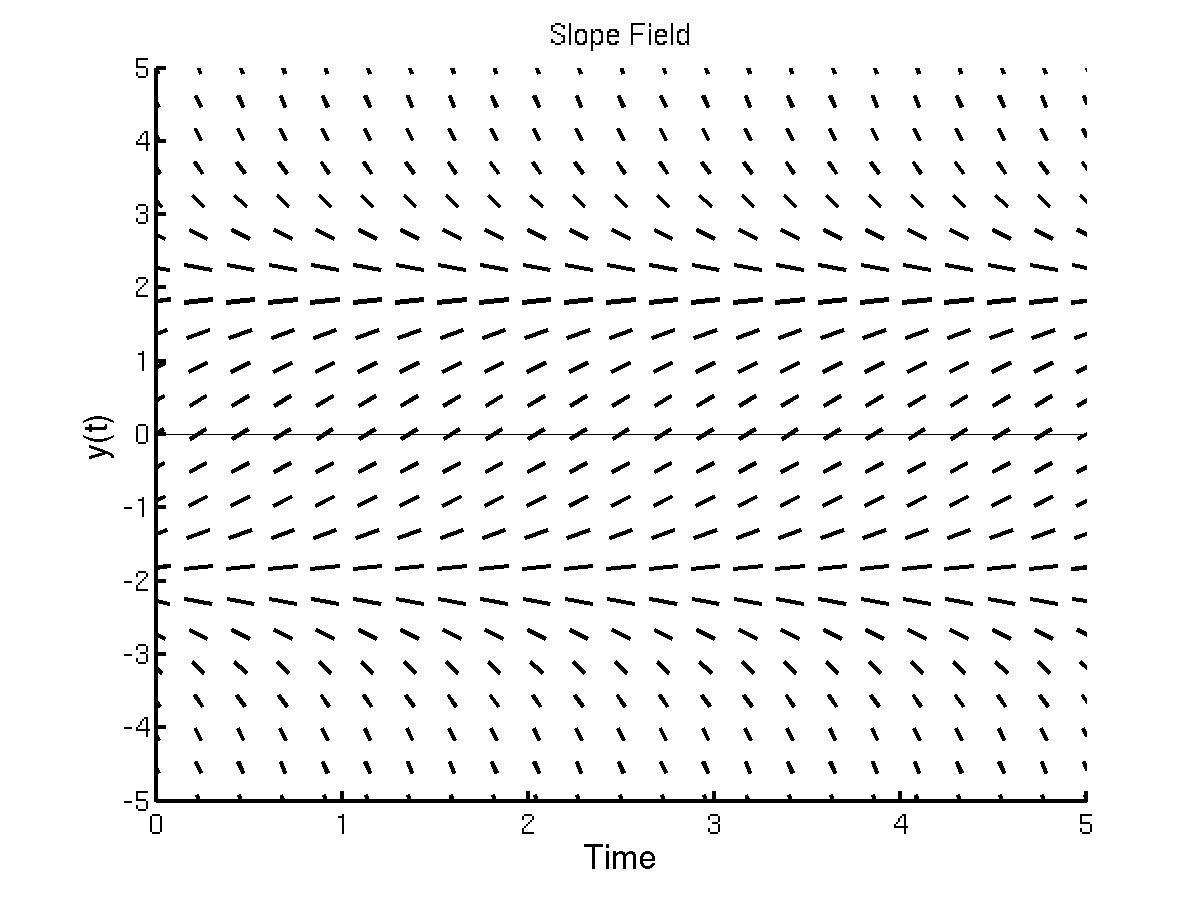
\includegraphics[height=4.0in]{sfStabilityWk1}

  \end{subproblem}

\end{problem}


\actTitle{The Chain Rule}
\begin{problem}
  \item Suppose that $3t+C=\ln(y(t))$ where $C$ is a constant. Solve
    the equation for $y(t)$.

    \vfill

  \item The function $y(t)$ depends on $t$. Use the chain rule to find
    the derivative of $\ln(y(t))$.
    \vfill

    \clearpage

  \item Show that the relationship $3t+C=\ln(y(t))$ can also be
    expressed as $y'=3y$.

    \vfill

  \item Show that for any constant $k$ the function
    \begin{eqnarray*}
      y(t) & = & k e^{5t}
    \end{eqnarray*}
    is a solution to the differential equation 
    \begin{eqnarray*}
      y' & = & 5y.
    \end{eqnarray*}
    \vfill

\end{problem}
